\section{ПАТТЕРНЫ ПОВЕДЕНИЯ}

Паттерны поведения связаны с алгоритмами и распределением обязанностей между объектами.

Речь в них идет не только о самих объектах и классах, но и о типичных
способах взаимодействия. Паттерны поведения характеризуют сложный поток
управления, который трудно проследить во время выполнения программы.
Внимание акцентировано не на потоке управления как таковом, а на связях между
объектами.

В паттернах поведения уровня класса используется наследование, чтобы распределить 
поведение между разными классами.

Различают паттерны поведения уровня классов и паттерны повендения уровня классов.
Паттерны поведения уровня классов:
\begin{itemize}
\item
  \textbf{<<шаблонный метод>>}, который представляет собой абстрактное определение алгоритма;
\item
  \textbf{<<интерпретатор>>}, который представляет грамматику языка в виде иерархии классов
  и реализует интерпретатор как последовательность операций над
  экземплярами этих классов;
\end{itemize}

Паттерны поведения уровня объектов:
\begin{itemize}
  
\item
  \textbf{<<посредник>>}, который находится между объектами-коллегами и
  обеспечивает косвенность ссылок, необходимую для разрывания лишних связей;

\item
  \textbf{<<цепочка обязанностей>>} дает возможность посылать запросы объекту не напрямую,
  а по цепочке <<объектов-кандидатов>>;

\item
  \textbf{<<стратегия>>} инкапсулирует алгоритм объекта;

\item
  \textbf{<<команда>>} инкапсулирует запрос в виде объекта,
  который можно передавать как параметр, хранить в списке истории 
  или использовать как-то иначе;

\item
  \textbf{<<состояние>>} инкапсулирует состояние объекта таким образом,
  что при изменении состояния объект может изменять поведение;

\item
  \textbf{<<посетитель>>} инкапсулирует поведение, которое в противном
  случае пришлось бы распределять между классами;

\item
  \textbf{<<итератор>>} абстрагирует способ доступа и
  обхода объектов из некоторого агрегата;

\end{itemize}

Стоит отметить, что для реализации паттернов поведения уровня классов используется
наследование, а для реализации паттернов поведения уровня объектов --- композиция.


\section{ПАТТЕРН ПОВЕДЕНИЯ <<СОСТОЯНИЕ>>}

\subsection{Назначение}

Паттерн <<состояние>> позволяет объекту варьировать свое поведение в зависимости
от внутреннего состояния.
Извне создается впечатление, что изменился класс объекта.

\subsection{Применимость}

Паттерн <<состояние>> следует использовать в следующих случаях:

\begin{itemize}
\item
  когда поведение объекта зависит от его состояния и должно изменяться во
  время выполнения;
\item
  когда в коде операций встречаются состоящие из многих ветвей условные
  операторы, в которых выбор ветви зависит от состояния.
\end{itemize}

\subsection{UML-диаграмма паттерна проктирования <<состояние>>}

Диаграмма классов паттерна проектирования <<состояние>> приведена
на рисунке~\ref{pic:UML_state}.

\begin{figure}[htbp]
  \centering
  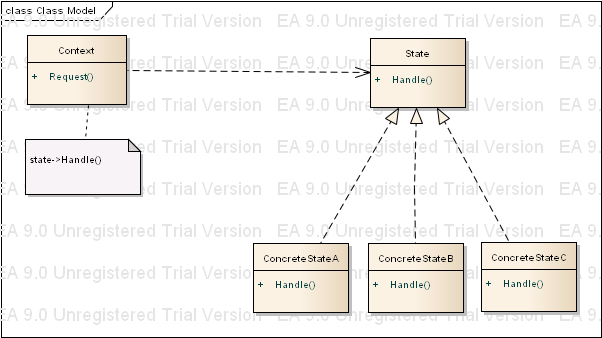
\includegraphics[width=150mm,height=92mm]{pic/class_model}
  \caption{UML-диаграмма паттерна <<состояние>>}
  \label{pic:UML_state}
\end{figure}

Рассмотрим классы, представленные на диаграмме.

\textbf{Context }(контекст):
\begin{itemize}
\item
  определяет интерфейс, представляющий интерес для клиентов;
\item
  хранит экземпляр подкласса ConcreteState, которым определяется
  текущее состояние;
\end{itemize}

\textbf{State }(состояние):
определяет интерфейс для инкапсуляции поведения, ассоциированного
с конкретным состоянием контекста Context.

\textbf{Подклассы ConcreteState } --- конкретные состояния:
каждый подкласс реализует поведение, ассоциированное с некоторым 
состоянием контекста Context.

\subsection{Отношения между классами}

\begin{itemize}
\item
  класс Context делегирует зависящие от состояния запросы текущему
  объекту ConcreteState;

\item
  Context может передать себя в качестве аргумента объекту State, который
  будет обрабатывать запрос. Это дает возможность объекту-состоянию
  при необходимости получить доступ к контексту;

\item
  Context --- это основной интерфейс для клиентов. Клиенты могут конфигурировать
  контекст объектами состояния State. Один раз сконфигурировав
  контекст, клиенты уже не должны напрямую связываться с объектами
  состояния;

\item
  либо Context, либо подклассы ConcreteState могут решить, при каких
  условиях и в каком порядке происходит смена состояний.
\end{itemize}


\subsection{Результаты использования паттерна}

Паттерн <<состояние>> помещает все поведение, ассоциированное с конкретным
состоянием, в отдельный объект. Поскольку зависящий от состояния код
целиком находится в одном из подклассов класса State, то добавлять
новые состояния и переходы можно просто путем порождения новых подклассов.

Логика, описывающая переходы между состояниями, больше не заключена
в монолитные операторы if или switch, а распределена между подклассами State.
При инкапсуляции каждого перехода и действия в класс состояние
становится полноценным объектом. Это улучшает структуру кода и проясняет его назначение.

\subsection{Пример использования}

В следующем примере приведен упрощенный вариант протокола TCP, в нем, конечно же,
представлен не весь протокол и даже не все состояния TCP-соединений.

Определение класса TCPConnection, который предоставляет интерфейс
для передачи данных и обрабатывает запросы на изменение состояния,
приведено на рисунке~\ref{lst:TCPConnection}.

\begin{lstlisting}[language=c++,caption=Класс TCPConnection,label=lst:TCPConnection]
class TCPOctetStream;
class TCPState;
class TCPConnection {
  public:
    TCPConnection();
    void ActiveOpen();
    void PassiveOpen();
    void Close();
    void Send();
    void Acknowledge();
    void Synchronize();
    void ProcessOctet(TCPOctetStream*);
  private:
    friend class TCPState;
    void ChangeState (TCPState*);
  private:
    TCPState* _state;
};

TCPConnection::TCPConnection () {
  _state = TCPClosed::Instance();
}

void TCPConnection::ChangeState (TCPState* s) {
  _state = s;
}

void TCPConnection::ActiveOpen () {
  _state->ActiveOpen(this);
}

void TCPConnection::PassiveOpen () {
  _state->PassiveOpen(this);
}

void TCPConnection::Close () {
  _state->Close(this);
}

void TCPConnection:Acknowledge () {
  _state->Acknowledge(this);
}

void TCPConnection::Synchronize () {
  _state->Synchronize(this);
}
\end{lstlisting}

В переменной-члене \_state класса TCPConnection хранится экземпляр
класса TCPState. Этот класс дублирует интерфейс изменения состояния,
определенный в классе TCPConnection.

TCPConnection делегирует все зависящие от состояния запросы хранимому
в \_state экземпляру TCPState. Кроме того, в классе TCPConnection существует
операция, с помощью которой в эту переменную можно записать указатель на
другой объект TCPState. Конструктор класса TCPConnection инициализирует
\_state указателем на состояние TCPClosed.

Определение абстрактного класса TCPState
приведено на рисунке~\ref{lst:TCPState}.
Каждая операция TCPState принимает экземпляр TCPConnection как параметр,
тем самым позволяя объекту TCPState
получить доступ к данным объекта TCPConnection и изменить состояние соединения.

\begin{lstlisting}[language=c++,caption=Класс TCPState,label=lst:TCPState]
class TCPState {
  public:
    virtual void Transmit(TCPConnection*, TCPOctetStream*);
    virtual void ActiveOpen(TCPConnection*);
    virtual void PassiveOpen(TCPConnection*);
    virtual void Close(TCPConnection*);
    virtual void Synchronize (TCPConnection*) ;
    virtual void Acknowledge (TCPConnection*) ;
    virtual void Send (TCPConnection* );
  protected:
    void ChangeState (TCPConnection*, TCPState*);
};

void TCPState::Transmit (TCPConnection*, TCPOctetStream*) { }
void TCPState::ActiveOpen (TCPConnection*) { }
void TCPState::PassiveOpen (TCPConnection*) { }
void TCPState::Close (TCPConnection*) { }
void TCPState::Synchronize (TCPConnection*) { }
void TCPState::ChangeState (TCPConnection* t, TCPState* s) {
  t->ChangeState(s) ;
}
\end{lstlisting}

В подклассах TCPState реализовано поведение, зависящее от состояния.
Соединение TCP может находиться во многих состояниях:
Established (установлено), Listening (прослушивание), Closed (закрыто) и т.д.,
и для каждого из них есть свой подкласс TCPState.

Определение и реализация подклассов TCPState приведены на рисунках~\ref{lst:TCPState_subclasses_declaration}~и~\ref{lst:TCPState_subclasses_realization}.

\begin{lstlisting}[language=c++,caption=Подклассы TCPState,label=lst:TCPState_subclasses_declaration]
  class TCPEstablished : public TCPState {
    public:
    static TCPState* Instanced;
    virtual void Transmit (TCPConnection*, TCPOctetStream*) ;
    virtual void Close (TCPConnection*) ;
  };
  class TCPListen : public TCPState {
    public:
    static TCPState* Instance();
    virtual void Send(TCPConnection*);
    // ...
  };
  class TCPClosed : public TCPState {
    public:
    static TCPState* Instanced;
    virtual void ActiveOpen(TCPConnection*);
    virtual void PassiveOpen(TCPConnection*);
    // ...
  };
\end{lstlisting}

\begin{lstlisting}[language=c++,caption=Примеры реализаций методов подклассов TCPState,label=lst:TCPState_subclasses_realization]
void TCPClosed::ActiveOpen (TCPConnection* t) {
  ChangeState(t, TCPEstablished::Instanced); }

void TCPClosed::PassiveOpen (TCPConnection* t) {
  ChangeState(t, TCPListen::Instance); }

void TCPEstablished::Close (TCPConnection* t) {
  ChangeState(t, TCPListen::Instance); }

void TCPEstablished::Transmit (TCPConnection* t, TCPOctetStream* o) {
  t->ProcessOctet(o); }

void TCPListen::Send (TCPConnection* t) { 
  ChangeState(t, TCPEstablished::Instance); }
\end{lstlisting}

В подклассах TCPState нет никакого локального состояния, поэтому их можно
 разделять, так что потребуется только по одному экземпляру каждого класса.
Уникальный экземпляр подкласса TCPState создается обращением к статической
операции Instance.

Материалы для ответа взяты из источника~\cite{gamma01}.